\documentclass[aspectratio=43]{beamer}
\usetheme{Madrid}
\usepackage[english]{babel}
\title{ETG Turbulence Isotropization}
\author[S. Tirkas]{Stefan Tirkas}
\institute[CIPS]{
    CIPS%
    \\%
    University of Colorado, Boulder%
} 
\date{\today}
\logo{
\includegraphics[width=.2\linewidth]{Images/BoulderLogo.png}}

\begin{document}
    
   \frame{\titlepage}
   
   \begin{frame}{Outline}
       \tableofcontents
   \end{frame}
   
   \section{Drift Wave Instabilities}
   
   \begin{frame}{Drift Wave Instabilities}
      \begin{itemize}
         \item Drift waves are most simply characterized as density, temperature and electrostatic potential fluctuations
         in low-$\beta$ plasmas.
         \vspace{5mm}
         \item Modes relevant to tokamak physics include ion-temperature-gradient modes (ITG), electron-temperature-gradient 
         modes (ETG), and collisionally-trapped electron modes (CTEM).
         \vspace{5mm}
         \item Low-frequency drift wave turbulence is largely responsible for the anomalous transport of plasma particles
         across magnetic field lines.
      \end{itemize}
   \end{frame}

   \begin{frame}{Ion-Temperature-Gradient Mode}
      \begin{figure}
         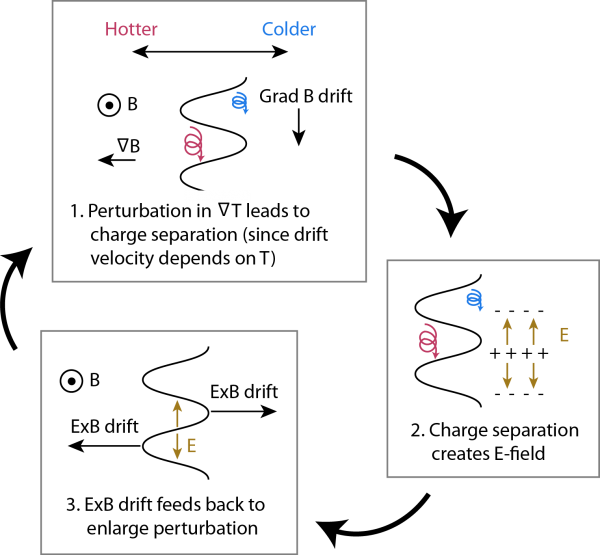
\includegraphics[scale=0.3]{Images/ITG_Instability.png}
         \caption{Simple pciture of ITG instability.}
      \end{figure}
   \end{frame}

   \begin{frame}{ETG Simulation in GENE}
      \begin{columns}
      \column{0.5\textwidth}
         \begin{figure}
            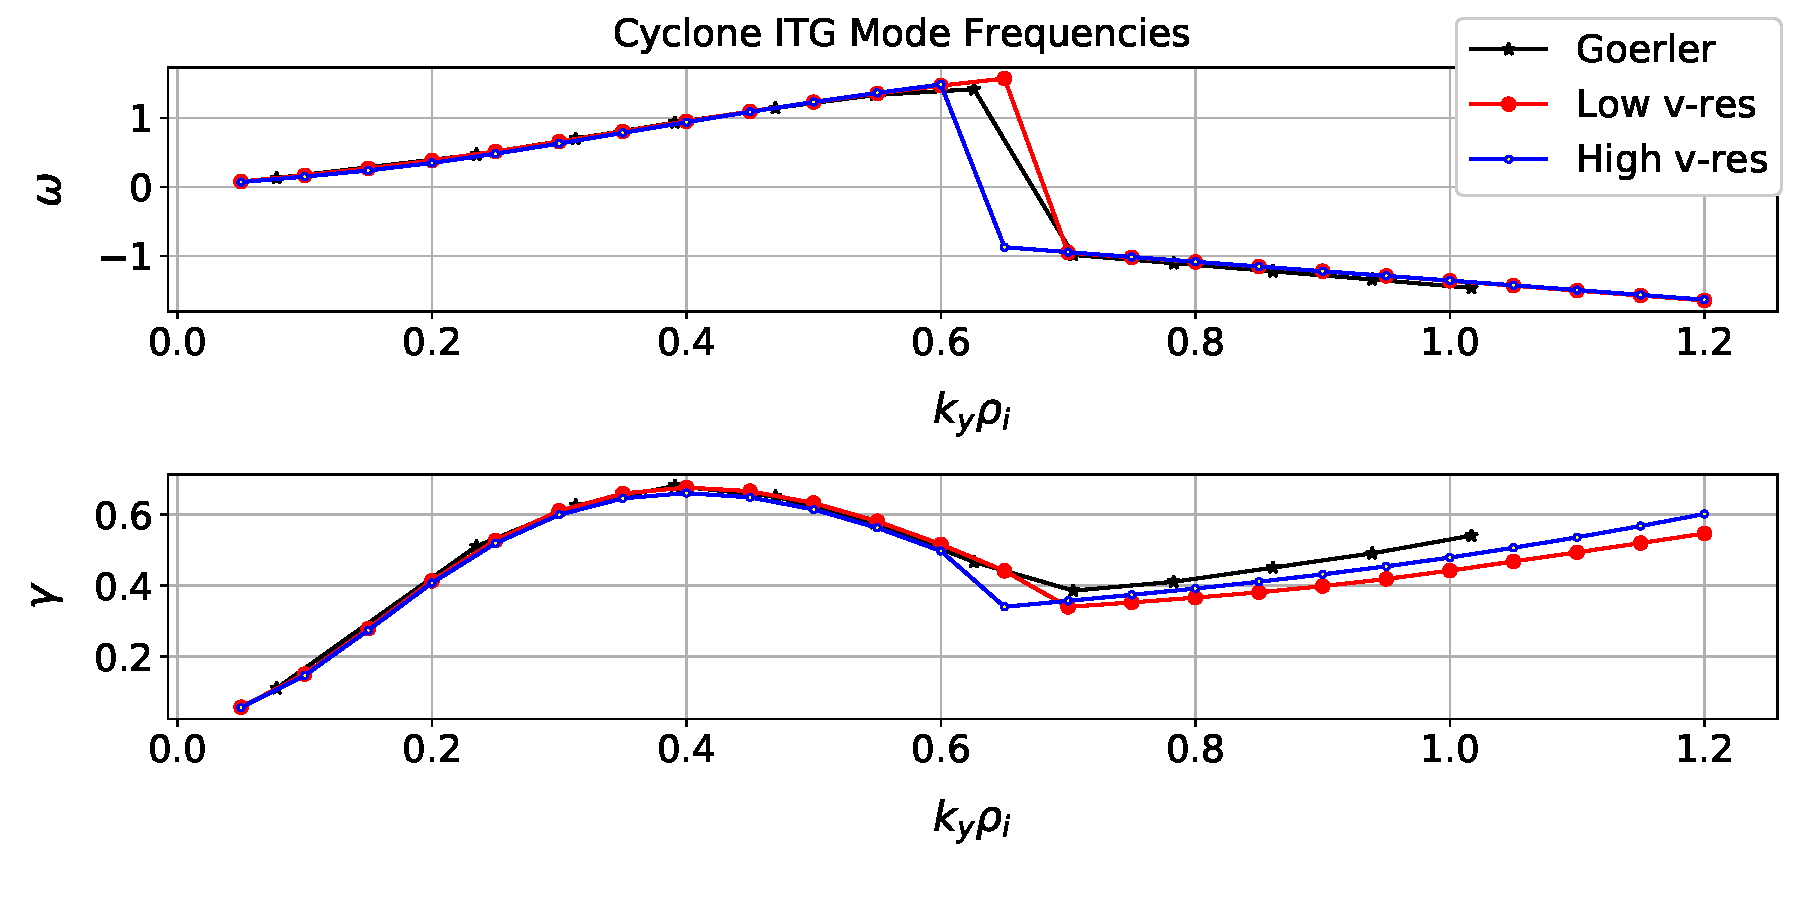
\includegraphics[width=.8\textwidth,height=.3\textheight]{Images/LinearITG_KinEl_GrowthRates.pdf}
            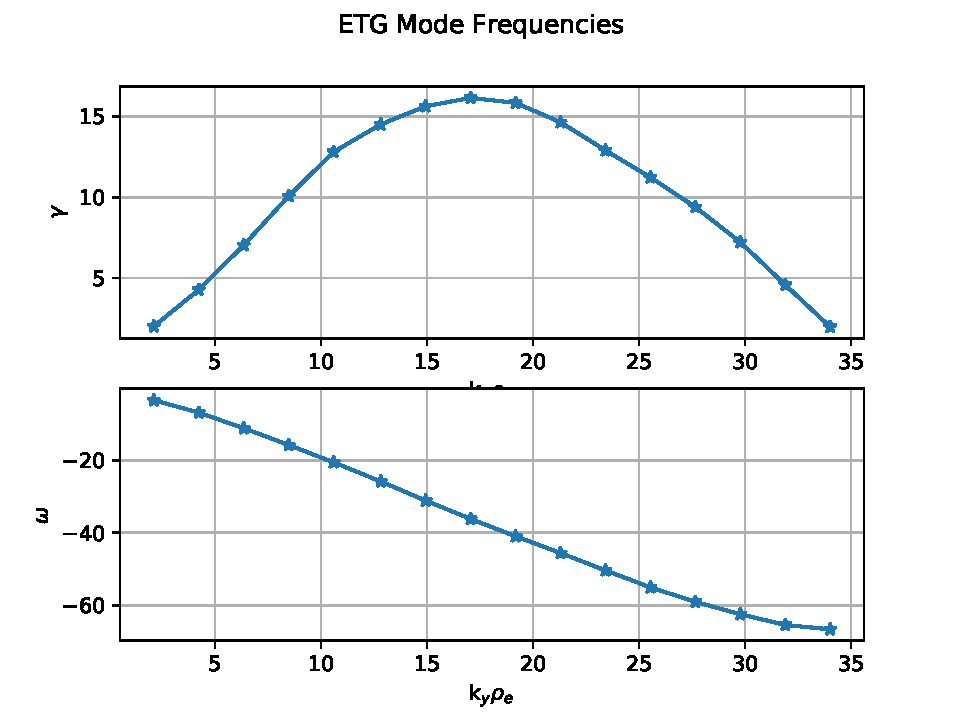
\includegraphics[width=.8\textwidth]{Images/GrowthRates_ETG.pdf}
         \end{figure}
      \column{0.5\textwidth}
      \end{columns}
   \end{frame}

   \begin{frame}
      \begin{columns}
      \column{0.5\textwidth}
         \begin{figure}
            \hspace*{-.3cm}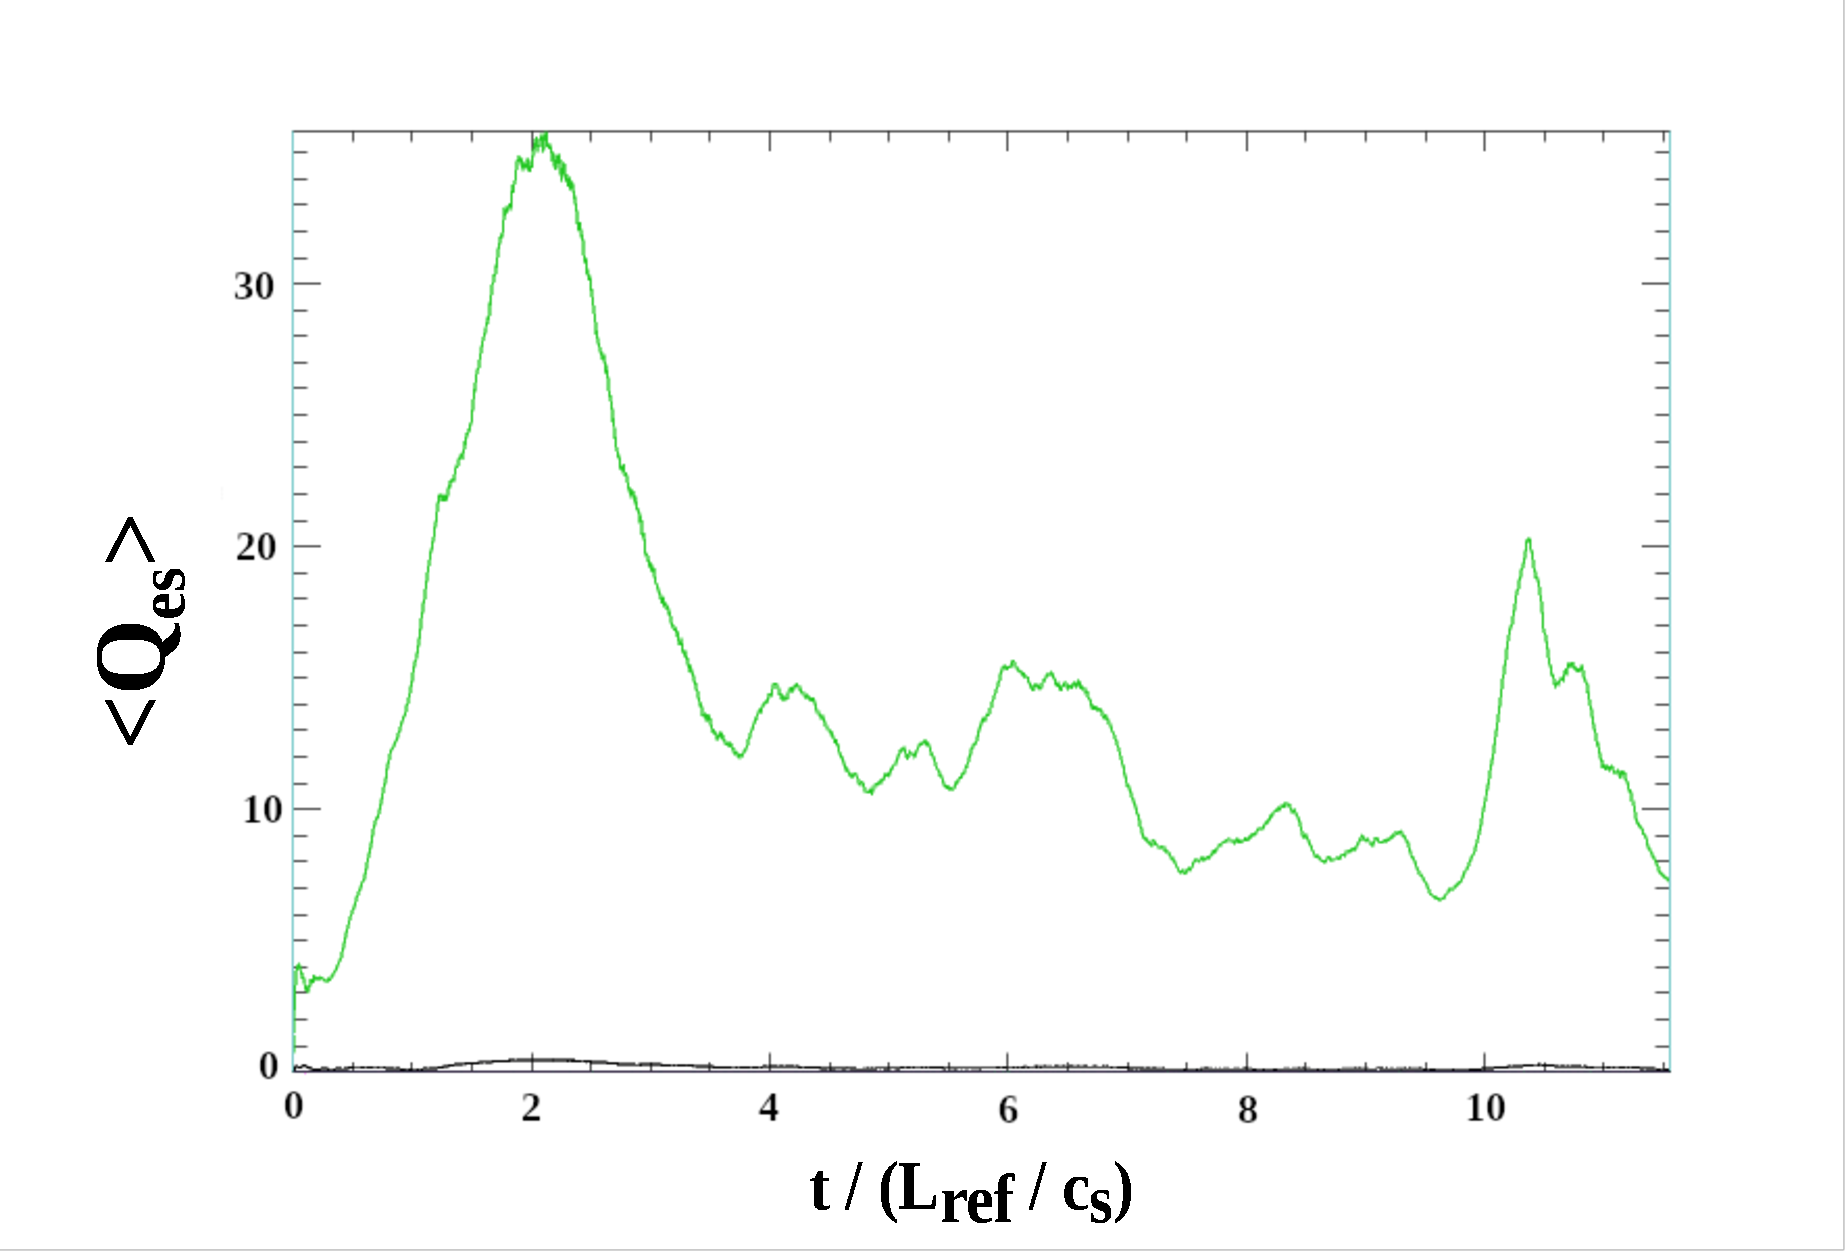
\includegraphics[scale=.2]{Images/etgHeatFlux.pdf}
            \hspace*{-.3cm}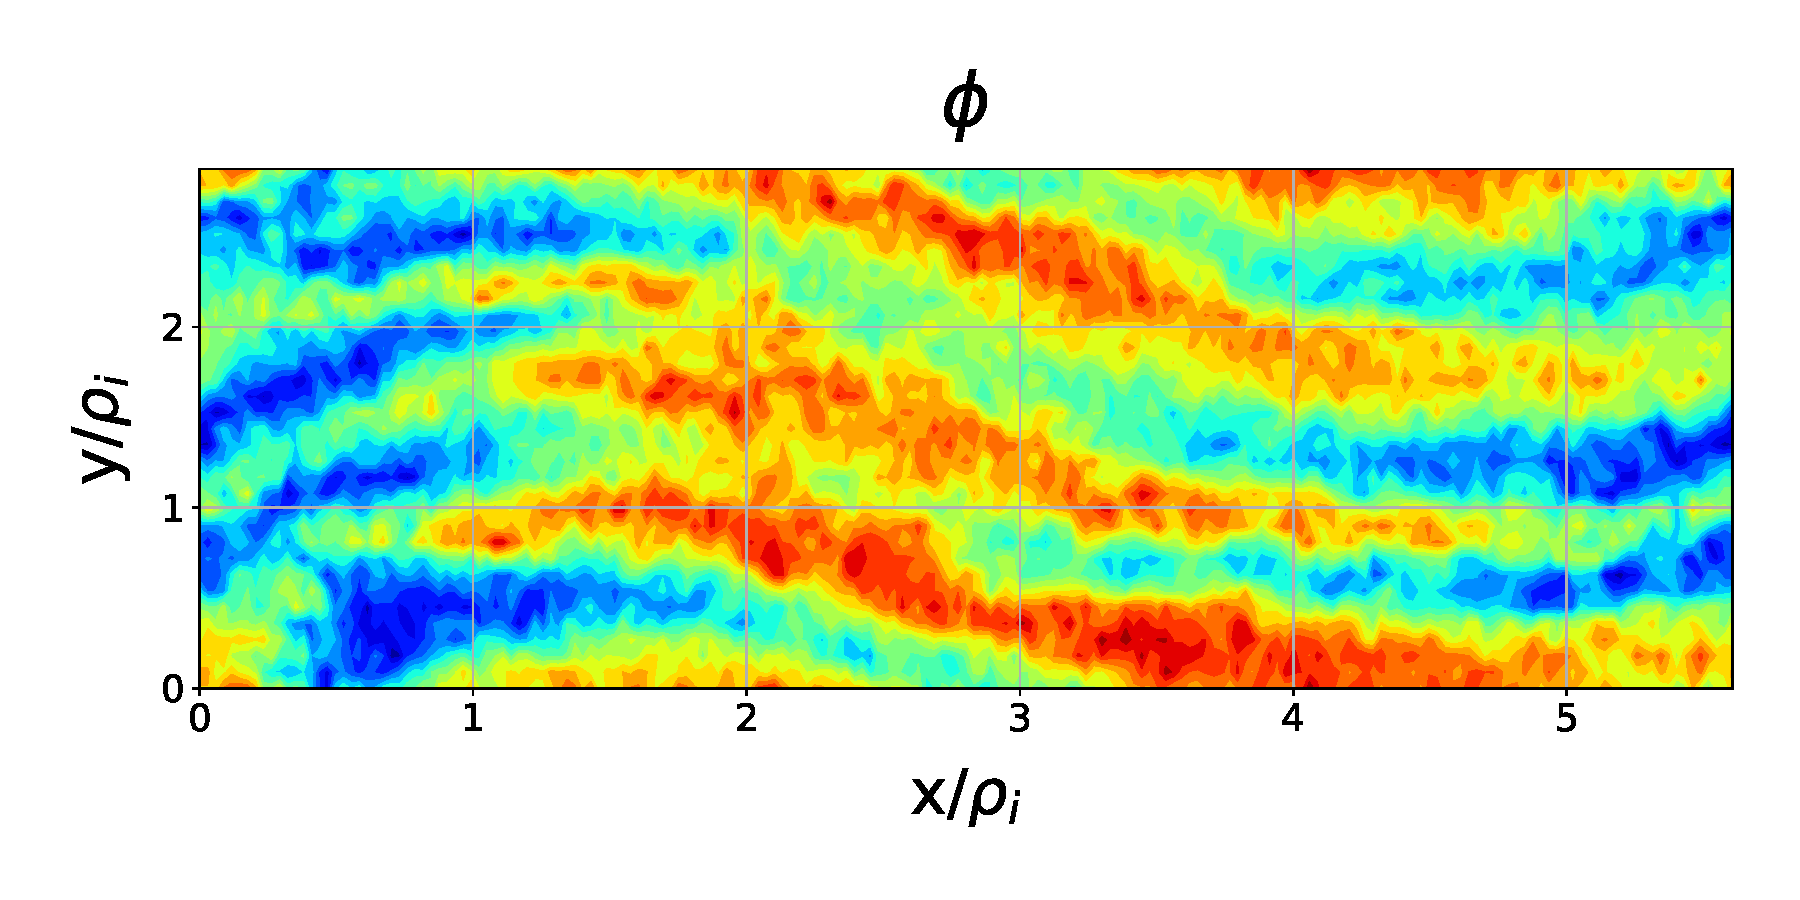
\includegraphics[scale=.2]{Images/genePhiETG_sat2.pdf}
         \end{figure}
      \column{0.5\textwidth}
      \end{columns}
   \end{frame}

   \section{Hasegawa-Mima Fluid Model}

   \begin{frame}{Hasegawa-Mima Fluid ETG Model}
      \begin{itemize}
         \item Partial differential equation derived from fluid continuity and momentum equations.
         \item Approximations made that are useful to describing  turbulence in tokamak plasmas.
         \begin{itemize}
            \item Cyclotron motion periods much smaller than time scales that quantities of interest change on ($B$,$\Phi$,$n$).
            \item Long length scales along $\hat{b}$-direction - $k_{\parallel}$ ignorable.
            \item Quasi-neutrality of particle densities is enforced.
            \item Isothermal equation of state, with adiabatic ions that have negligible temperatures.
         \end{itemize}
         \item Shown to cause isotropic behavior for long wavelength modes as well as an inverse energy-cascade.
      \end{itemize}
   \end{frame}

   \begin{frame}{Hasegawa-Mima Equations}
      \quad We start with the fluid continuity and momentum equations, where we have already taken the ion approximations discussed
   on the previous slide:
      \begin{equation}
         \frac{\partial n_e}{\partial t} + \nabla\cdot\left(n_e\vec{v}_e\right) = 0,
      \end{equation}
      %
      \begin{equation}
            m_e\frac{d\vec{v}_e}{dt} = \left(1+\tau\right)e\nabla\delta\Phi - \frac{e}{c}\vec{v}_e\times\vec{B}-\frac{\nabla P_e}{n_e}\;.
      \end{equation}
   We break equation (2) up into parallel and perpendicular components, and break up $\vec{v}_e$ in terms of higher and lower order terms to find,
      \begin{equation}
      \begin{aligned}
         \vec{v}_{e,0} &= \vec{v}_{\parallel} + \vec{v}_{\perp,0} = \vec{v}_{\parallel} + \left(1 + \tau\right)\vec{v}_E + \vec{v}_D \\
         \vec{v}_{e,1} &= \vec{v}_{\perp,1}
      \end{aligned}
      \end{equation}
   \end{frame}

   \begin{frame}{Hasegawa-Mima Equations}
      \quad Taking the standard electron dyanamic normalization,
      \begin{equation}
      \begin{aligned}
         \Phi    = \frac{e\delta\Phi}{T_i},&\; -\frac{1}{r_n}=\frac{\partial_x n_e}{n_e},\; -\frac{1}{r_t}=\frac{\partial_x T_e}{T_e},\; \eta_e=\frac{r_n}{r_t},\; \\
         \rho_e &= \sqrt{\frac{\tau m_e}{m_i}}\rho_i,\; \vec{x} = \frac{\vec{x}}{\rho_e},\; t=\frac{\rho_e}{r_n}\omega_{ce}t
      \end{aligned}
      \end{equation}
   and plugging into equation () gives the form of the H-M ETG model,
      \begin{equation}
      \begin{aligned}
         &-(1-\frac{1+\tau}{2\tau}\nabla_{\perp}^2)\partial_t\Phi + \frac{1+\tau}{2\tau}\frac{r_n^2}{\rho_e^2}\partial_t^{-1}\nabla_{\parallel}^2\Phi
          + \frac{(1+\tau)(1+\eta_e)}{4\tau}\partial_y\nabla_{\perp}^2\Phi \\
         &+ \frac{1+\eta_e}{2\tau}\partial_y\Phi + \frac{(1+\tau)^2}{\tau^2}\frac{r_n}{4\rho_e}(\hat{b}\times\nabla_{\perp}\Phi\cdot\nabla_{\perp})\nabla_{\perp}^2\Phi = 0\;.
      \end{aligned}
      \end{equation}
   \end{frame}

   \begin{frame}{Hasegawa-Mima Equations}
      \quad Finally we drop the parallel gradient term since $k_{\parallel}^2/k_{\perp}^2 \sim \epsilon^2$, and simplify the bracketed expression to find the final
      form of our model,
   \end{frame}

   \begin{frame}{Pseudo-Spectral Solver}
      \quad Equation () is solved numerically using the pseudo-spectral method with a 4th-order Runge-Kutta time advancement. We take the Fourier transform of the equation, but
   leave the non-linear terms in real space. We can solve for $\zeta_{x,y}$ and $\Phi_{x,y}$ in Fourier space, inverse transform to real space, take the necessary non-linear products,
   and transform the final result back to Fourier space to carry out the time advancement.
   \end{frame}

   \begin{frame}{ETG H-M Results}
      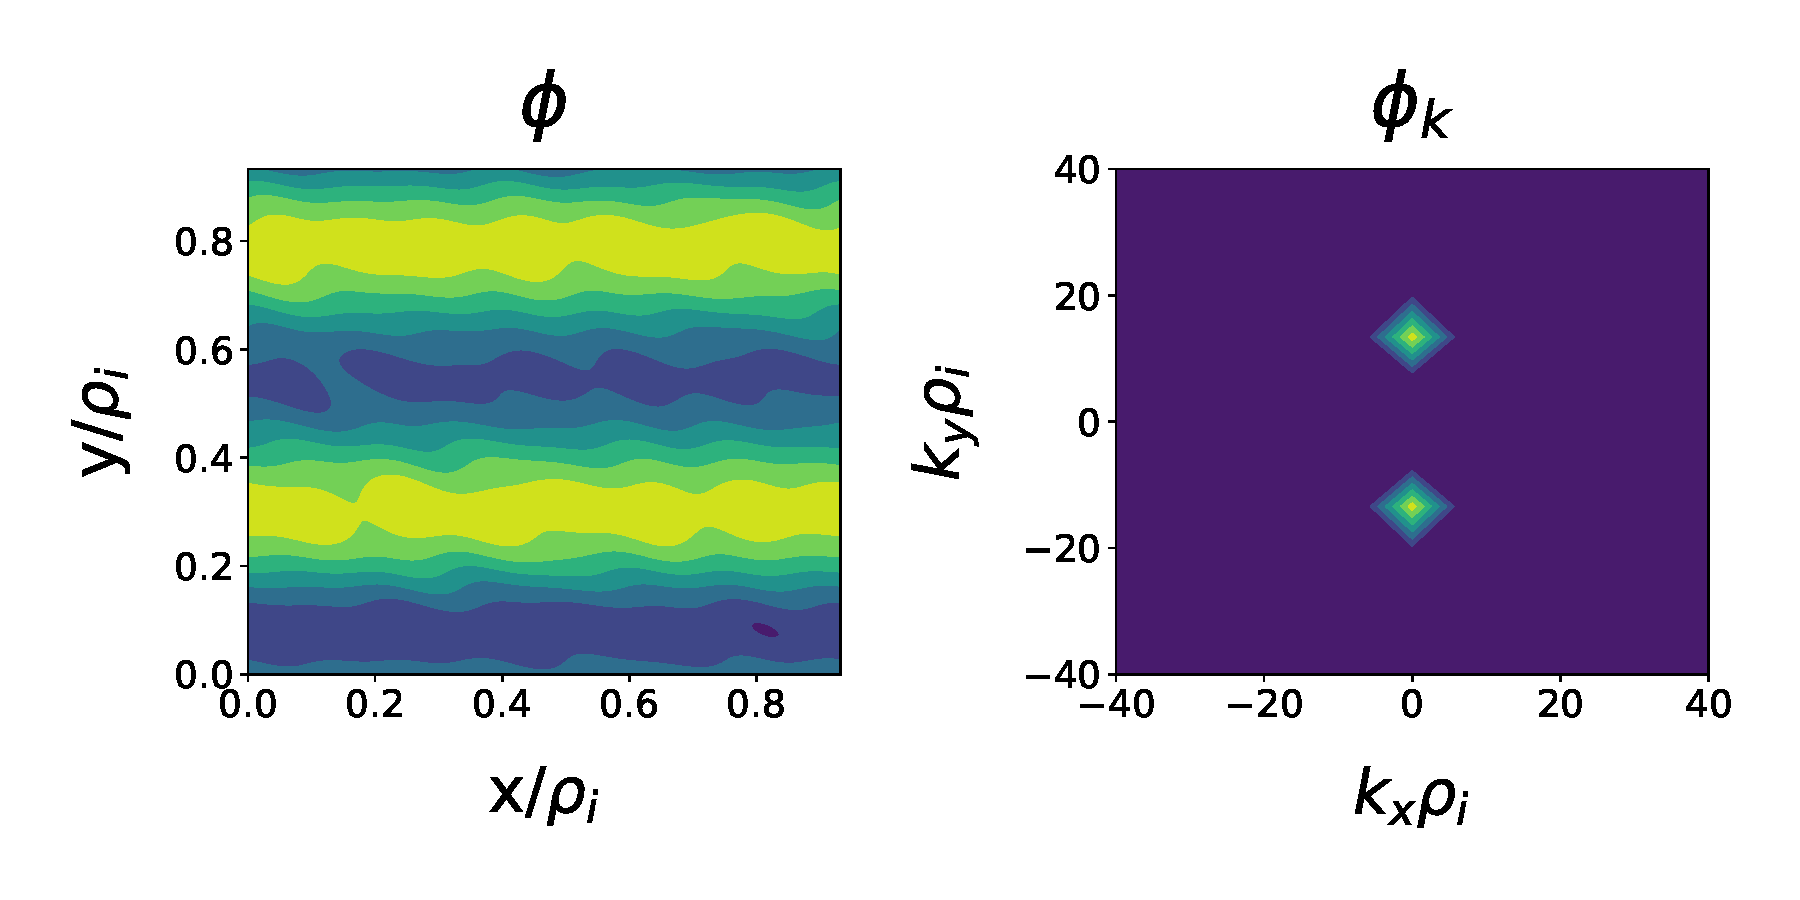
\includegraphics[scale=.25]{Images/hmPhiETG_init.pdf}
      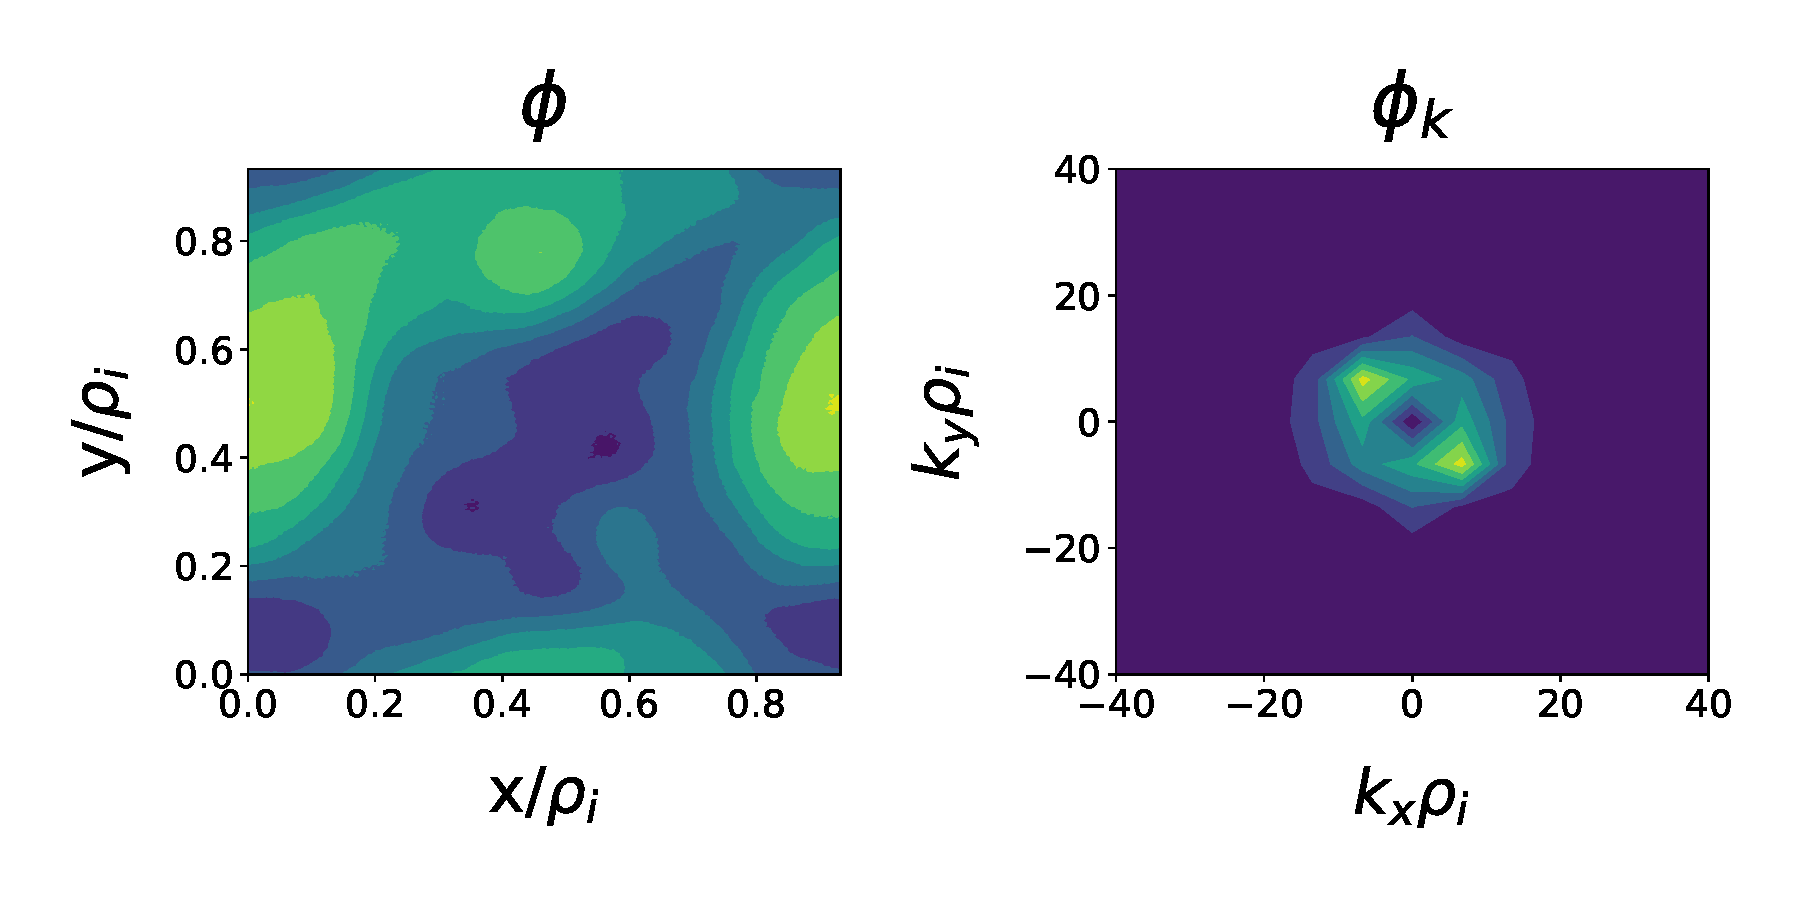
\includegraphics[scale=.25]{Images/hmPhiETG_iso.pdf}
   \end{frame}

   \begin{frame}{GENE ETG Streamer Test}
      
   \end{frame}

   \begin{frame}{Effects of Isotropization}
      
   \end{frame}

   \section{Zonal Flow Excitation}

   \begin{frame}{Zonal Flow Excitation}
   \end{frame}
   
   \section*{Acknowledgments} %You can remove this if you do not want to use it
      \begin{frame}{Acknowledgments}
          The author is extremely thankful to Prof. Antônio F. R. T. Piza for the short, yet wonderful, conversations about this seminar.
      \end{frame}
   
   \section*{References}
      %\nocite{Djairo} \nocite{PhilPanof} \nocite{Fleming} \nocite{Shankar}
      \begin{frame}{References}
          %\printbibliography
      \end{frame}

\end{document}